\documentclass[fontsize=11pt, parskip=half]{scrartcl}

\usepackage{ngerman}
\usepackage[utf8]{inputenc}
\usepackage[T1]{fontenc}
\usepackage{graphicx}
\usepackage{enumitem}
\usepackage{amsmath}
\usepackage{amssymb}
\usepackage{hyperref}
\usepackage{pgfplots}
\setlength{\parindent}{0em}

% set section in CM
\setkomafont{section}{\normalfont\bfseries\Large}
\makeatletter
\renewcommand\sectionlinesformat[4]{%
  \Ifstr{#1}{section}
    {\@hangfrom{\hskip #2}{#4#3}}
    {\@hangfrom{\hskip #2#3}{#4}}% original definition for subsection, subsubsection
}
\makeatother
\renewcommand\sectionformat{\enskip\thesection\autodot}

%own commands
\newcommand{\Z}{\mathbb{Z}}
\newcommand{\Q}{\mathbb{Q}}
\newcommand{\R}{\mathbb{R}}
\newcommand{\C}{\mathbb{C}}
\newcommand{\N}{\mathbb{N}}
\newcommand{\E}{\mathbb{E}}
\renewcommand{\d}{\operatorname{d}}

\renewcommand{\vec}[1]{\boldsymbol #1}

\begin{document}

%% Headline
\noindent
\begin{tabular}{l}
    \textbf{Analysis und Lineare Algebra} \\    
    Prof. Dr. Jonas Offtermatt
\end{tabular}
\hfill 
\includegraphics[width=2cm]{DHBW.pdf}\\
\rule{\textwidth}{0.5pt}

%%

%% Title
\begin{center}
    \Large
    \textbf{Übungsblatt 4 Differentialrechnung mehrerer Veränderlicher}
\end{center}
%%
\section{Aufgabe}
Visualisieren Sie folgende mehrdimensionale Funktionen:
\begin{enumerate}[label=\alph*)]
    \item $f(x,y) = x^2 + y^2$
    \item $f(x,y) = 36 + 6x -x^2 + 10 y - y^2$
    \item $f(x,y) = \frac{1}{2}\sqrt[3]{x y^2}$
    \item $f(x,y) = \cos (\sqrt{x^2 + y^2})$
\end{enumerate}
Verwenden Sie hierfür ein Online-Tool Ihrer Wahl, bspw: 

\url{https://www.geogebra.org/classic#3d}

\section{Aufgabe}
Man kann Funktionen mehrerer Veränderlicher auch von Hand mittels eines Höhenlinienplots (Contour-Plot) visualisieren. 
Beispiel:

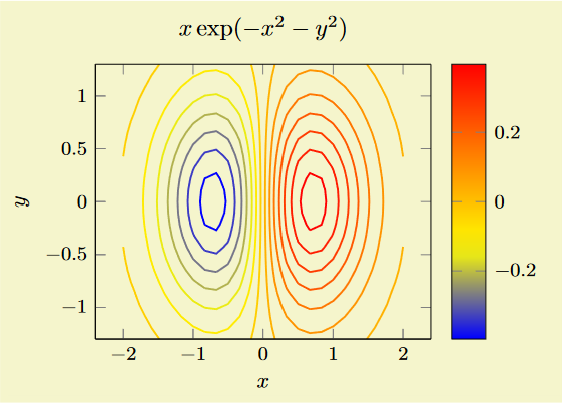
\includegraphics{countourplot.png}


Um diese zu erzeugen, löst man die Formel $f(x,y) = c$, mit $c \in \R$, nach $y$ auf. Dann setzt man $c = 0,1,2,..$ und kann so für verschiedene $x$-Werte den entsprechenden $y$-Wert bestimmen. Zeichnet man die verschiedenen Höhenlinien mit verschiedenen Farben (bspw. $c=0$ mit blau, $c=1$ mit gelb, $c= 2$ mit rot) ergibt sich ein farbliches Höhenbild.

Erstellen Sie einen Höhenlinien-Plot für die Funktion $f(x,y) = x^2 + y^2$.


\section{Aufgabe}
Die Höhe eines Geländes werde durch die Funktion $f(x,y) = 36 + 6x -x^2 + 10 y - y^2$ modelliert.
\begin{enumerate}[label=\alph*)]
    \item Gibt es auf diesem Gelände ein globales Maximum/Minimum? Wo liegt dieses?
    \item Der Meeresspiegel entspreche dem Höhenniveau $0$. Welche Punkte des Geländes liegen auf Meereshöhe?
\end{enumerate}


\section{Aufgabe}
Bestimmen Sie alle partiellen Ableitungen erster und zweiter Ordnung folgender Funktionen:
\begin{enumerate}[label=\alph*)]
    \item $f(x_1,x_2) = 2x_1^2+x_1^4x_2^2$
    \item $f(x_1,x_2) = \sin ( x_1)\cdot \cos (x_2)$
    \item $f(x_1,x_2) = \sqrt{1-x_1^2-x_2^2}$
\end{enumerate}

\section{Aufgabe}
Untersuchen Sie die Funktion $f(x,y)= 2x ^2 + y^2+xy+x-5y$ auf Extremwerte.

\section{Aufgabe}
Die Firma Seeblick GmbH vermiete Hotelzimmer zu zwei unterschiedlichen Preisen $p_1$ und $p_2$. Für den Umsatz
der Firma gelte folgende Umsatzfunktion:
\[U(p_1,p_2) = = 200p_1 +180p_2 -2p^2_1 +2p_1 p_2 -3p^2_2
    \]
\begin{enumerate}[label=\alph*)]
    \item Bestimmen Sie die partiellen Ableitungen nach $p_1$ und $p_2$ von $U$.
    \item Welche Preise $p_1,p_2$ sollten gewählt werden um den Umsatz zu maximieren?
    \item Skizzieren Sie Funktion und überprüfen Sie ihr Ergebnis aus dem vorigen Teil.
\end{enumerate}    

\end{document}